\chapter{Introduction}

%Provide a short summary of the whole PhD thesis:
% -Introduction to QC & CQED
% -Building Blocks of Superconducting Quantum Processors
% -Realization of a Two-Transmon QP
% -Tune-Up & Characterization of the Universal Two-Qubit Gate
% -Grover's Algorithm: Introduction & Background
% -Implementation on the Two-Qubit Processor
% -Design of a Scalable QC Architecture

\section{Quantum Computing \& Circuit Quantum Electrodynamics}

\begin{figure}
	\centering
		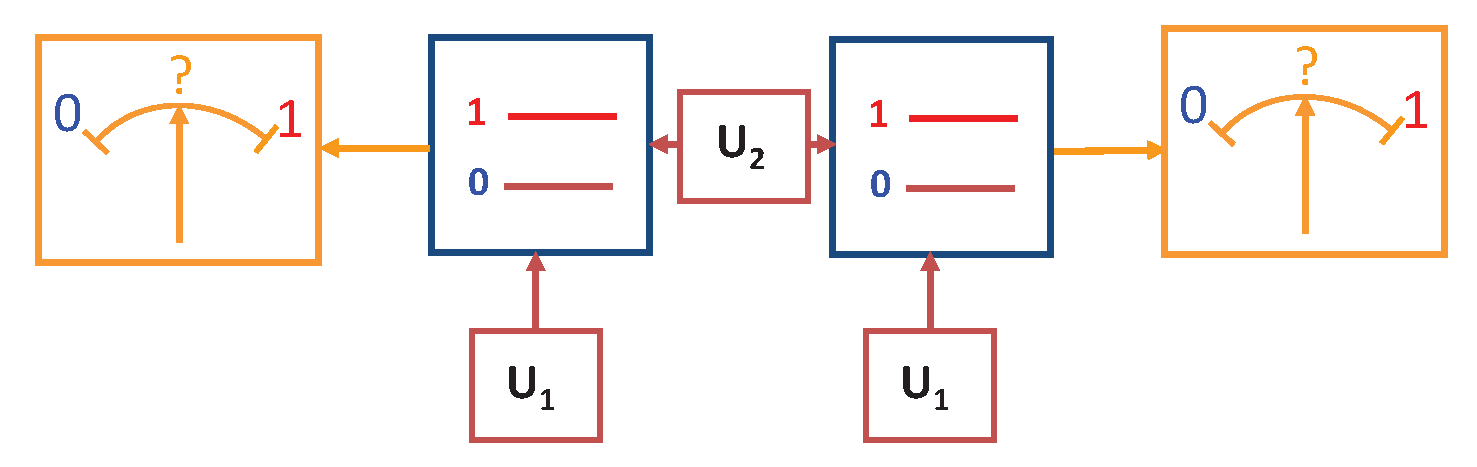
\includegraphics[width=0.8\textwidth]{./material/papers/grover/submission1/Fig1}
	\caption[Blueprint of a two-qubit quantum processor]{The blueprint of a two-qubit quantum processor. Shown are two qubits that can be individually manipulated ($U_1$) and are connected by a universal two-qubit gate $U_2$. Each of the qubits can be read out individually.}
	\label{fig:qubit_processor_blueprint}
\end{figure}

This thesis presents experiments performed on a superconducting Two-Qubit quantum processor. The main goal of this work was to demonstrate a possible quantum computing architecture using superconducting qubits that follows the canonical blueprint of a Two-qubit quantum processor, as given by the four criteria of \cite{divincenzo_physical_2000} and as shown in fig. \ref{fig:qubit_processor_blueprint}. By this definition a universal quantum computer is a register of quantum bits -- or qubits -- on which one can perform universal single- and two-qubit quantum gates, read out the state of each qubit individually and with high fidelity and reset the qubit register to a well-defined state.

Implementing this allegedly simple list of requirements in a system of superconducting qubits has been a major research challenge during the last decade. After the first demonstration of coherent quantum dynamics in a superconducting charge-based qubit by \cite{nakamura_coherent_1999}, a broad research field on superconducting quantum bits has sprung up. In the years following Nakamuras initial experiment, several types of superconducting qubits were proposed and realized using e.g. the superconducting phase \citep{martinis_energy-level_1985,martinis_rabi_2002} across a Josephson junction or the magnetic flux \citep{mooij_josephson_1999,chiorescu_coherent_2003} inside a superconducting ring interrupted by one or several Josephson junctions as the dominant quantum variable. An important result on the way to robust superconducting qubits was the development of the so-called {\it Quantronium} qubit by \cite{vion_manipulating_2002}, which demonstrated for the first time a quantum-mechanical coherence time larger than 1 $\mu s$ by operating a Cooper pair box at a sweet spot in a regime where the charging and Josephson phase energies of the system are of comparable value. This invention made it possible to perform for the first time robust, NMR-like quantum operations using a superconducting qubit \citep{collin_nmr-like_2004}. In 2004, the development of a new type of qubit, the so called {\it Transmon} by \cite{wallraff_strong_2004} achieved again a drastic improvement by operating a Cooper pair box in the phase regime and thus rendering the resulting qubit almost insensitive to charge noise. In addition, by embedding the qubit in a superconducting coplanar waveguide (CPW) resonator it is possible to protect it from external sources of electrical noise and to use the shift of the resonance frequency of the resonator caused by a dirspersive interaction with the qubit for reading out the qubit state\citep{blais_cavity_2004}. Using this so-called {\it circuit quantum electrodyanmics} (CQED) architecture, quantum gates and algorithms with up to four qubits have been implemented, demonstrating multi-qubit entanglement \citep{dicarlo_preparation_2010}and simple quantum algorithms \citep{dicarlo_demonstration_2009}.

\todo{Think about moving the section on 3D-CQED directly after this one since this would probably be more logical}

In parallel to this, the development of reliable quantum-limited amplifiers based on nonlinear superconducting resonators by \question{Should I mention Michel here?}I. Siddiqi \citep{siddiqi_rf-driven_2004} complemented the CQED architecture by providing a fast and high-fidelity readout scheme for Transmon qubits \citep{siddiqi_dispersive_2006,mallet_single-shot_2009} and for the amplification of quantum signals in general\todo{Add more citations here}. These quantum-limited amplifiers and detectors made it possible to directly observe quantum jumps in superconducting qubits \citep{vijay_observation_2011} and to implement quantum feedback in superconducting circuits\todo{Add reference to quantum feedback paper as soon as it appears}.

Recently, the development of a CQED architecture combining Transmon qubits with 3D superconducting resonator cavities instead of 1D coplanar waveguide resonators, as pioneered by \cite{paik_observation_2011}, resulted in an increase of qubit lifetimes of almost two orders of magnitude, with measured $T_1$ qubit relaxation times as high as $80 \; \mu \mathrm{s}$\todo{verify this!} and decoherence times at a comparable time scale. This increase in coherence times made possible the realization of high-fidelity quantum gates and qubit readout schemes \todo{add references!} as well as elemental quantum feedback and error correction schemes, thus bringing quantum computing using superconducting qubits almost within experimental reach.\todo{expand this section as soon as new relevant material appears, include recent IBM, Yale}

The research presented in this thesis wants to complement the CQED architecture by combining a multi-qubit architecture with a single-shot, individual-qubit readout scheme, thus aiming to develop a viable architecture for the implementation of a superconducting quantum computer using Transmon qubits. 

The first part of this thesis discusses therefore the realization of a superconducting quantum processor based on Transmon qubits and using an individual-qubit, single-shot readout scheme. We demonstrate elemental single- and two-qubit quantum operations on this processor and use it to implement a simple quantum algorithm that demonstrates quantum speed-up. Afterwards, we discuss the realization of a four-qubit quantum processor within a more scalable architecture that fulfills -- to different degrees -- all of the diVincenzo criteria and which could possibly be extended to a larger number of qubits.

\section{Realizing a Two-Qubit Quantum Processor}

\begin{figure}[ht!]
	\centering
		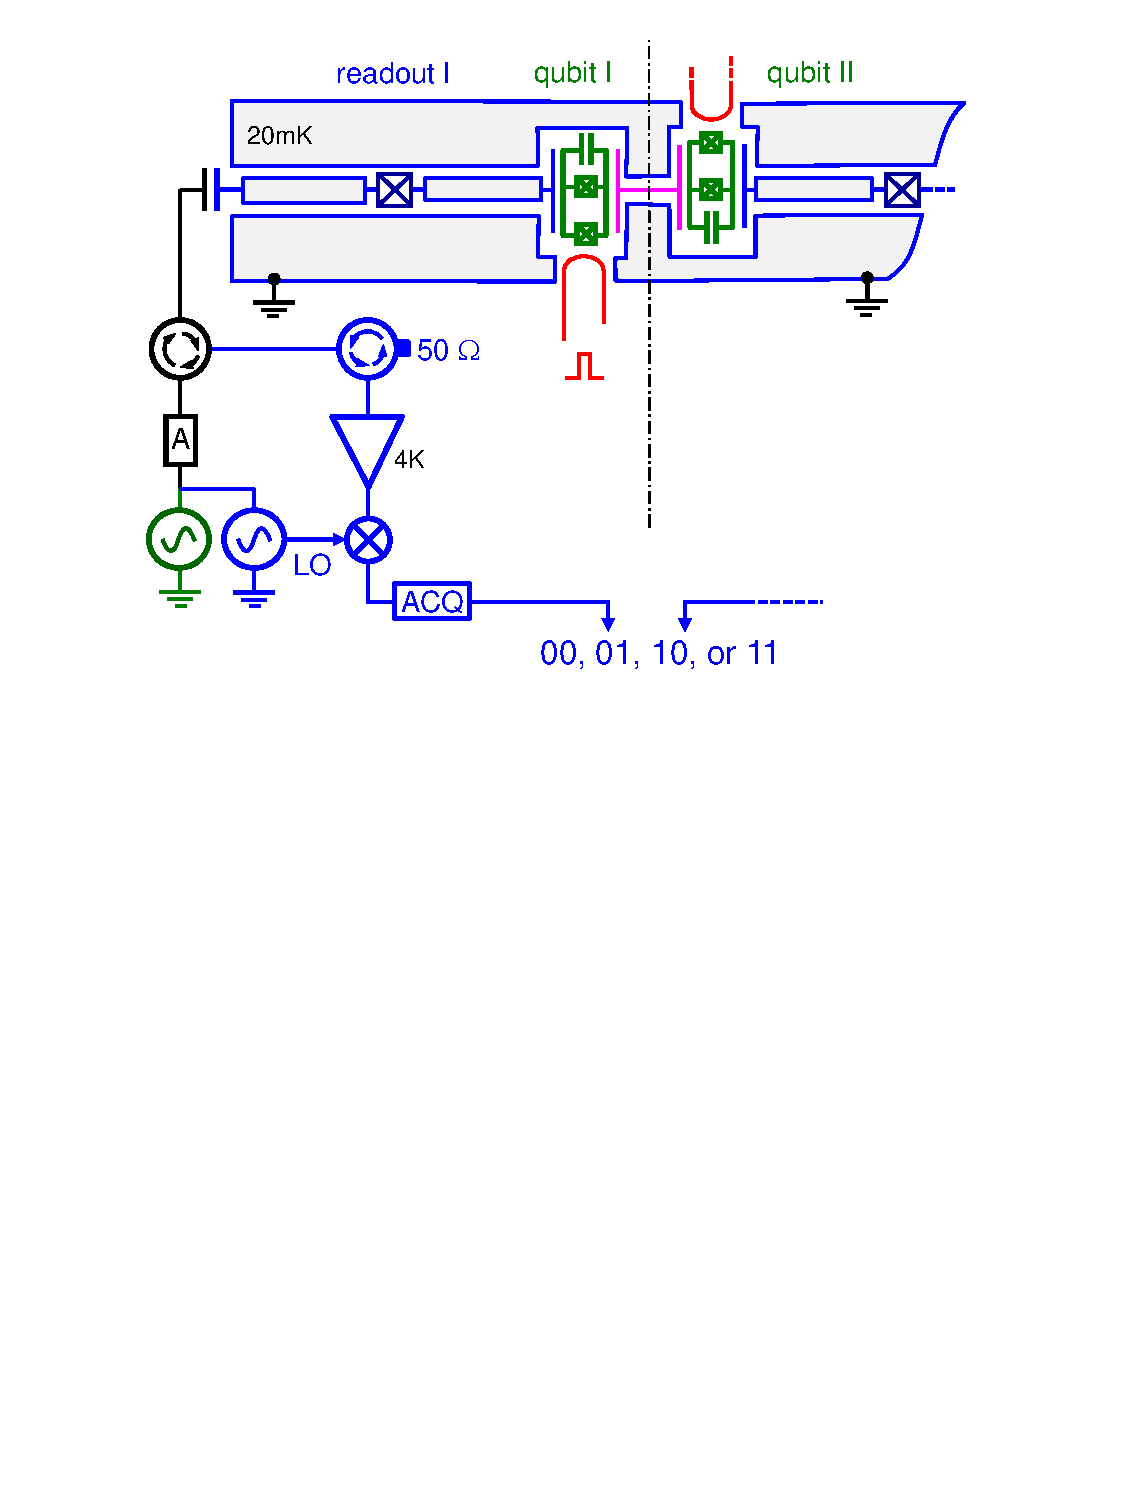
\includegraphics[width=0.75\textwidth]{./material/papers/grover/figures/2_qubit_processor_schematic}
	\caption[Circuit schematic of the realized two-qubit processor]{Circuit schematic of the two-qubit processor realized in this work, showing the two qubits in green, the qubit readouts in blue and the fast flux lines in red. Each qubit is embedded in its own nonlinear readout resonator and can be driven and read out through an individual microwave line.}
	\label{fig:two_qubit_processor_schematic}
\end{figure}

The quantum processor implemented in this work is shown in fig. \ref{fig:two_qubit_processor_schematic}. It consists of two superconducting quantum bits of the Transmon-type, each equipped with its own drive and readout circuit. The qubit readout is realized by using a nonlinear coplanar-waveguide resonator which serves as a Josephson bifurcation amplifier (JBA) and allows a high-fidelity, single-shot readout of the qubit state. Each qubit can be manipulated by driving it with microwave pulses through its readout resonator, allowing robust single-qubit operations. In addition, the qubit frequencies can be tuned individually by fast flux lines, which allows us to change the frequency each qubit over a range of several GHz. The coupling between the two qubits is realized through a fixed capacitor that directly connects the two qubits and implements a fixed $\sigma_{xx}$-type qubit-qubit coupling. This allows to implement two-qubit gates and to generate entangled two-qubit states. We use this processor to test Bell's inequality, implement an universal two-qubit gate and perform a simple quantum algorithm that demonstrates quantum speed-up, as will be discussed in the following sections.

\section{Demonstrating Simultaneous Single-Shot Readout}

\begin{figure}[ht!]
	\centering
		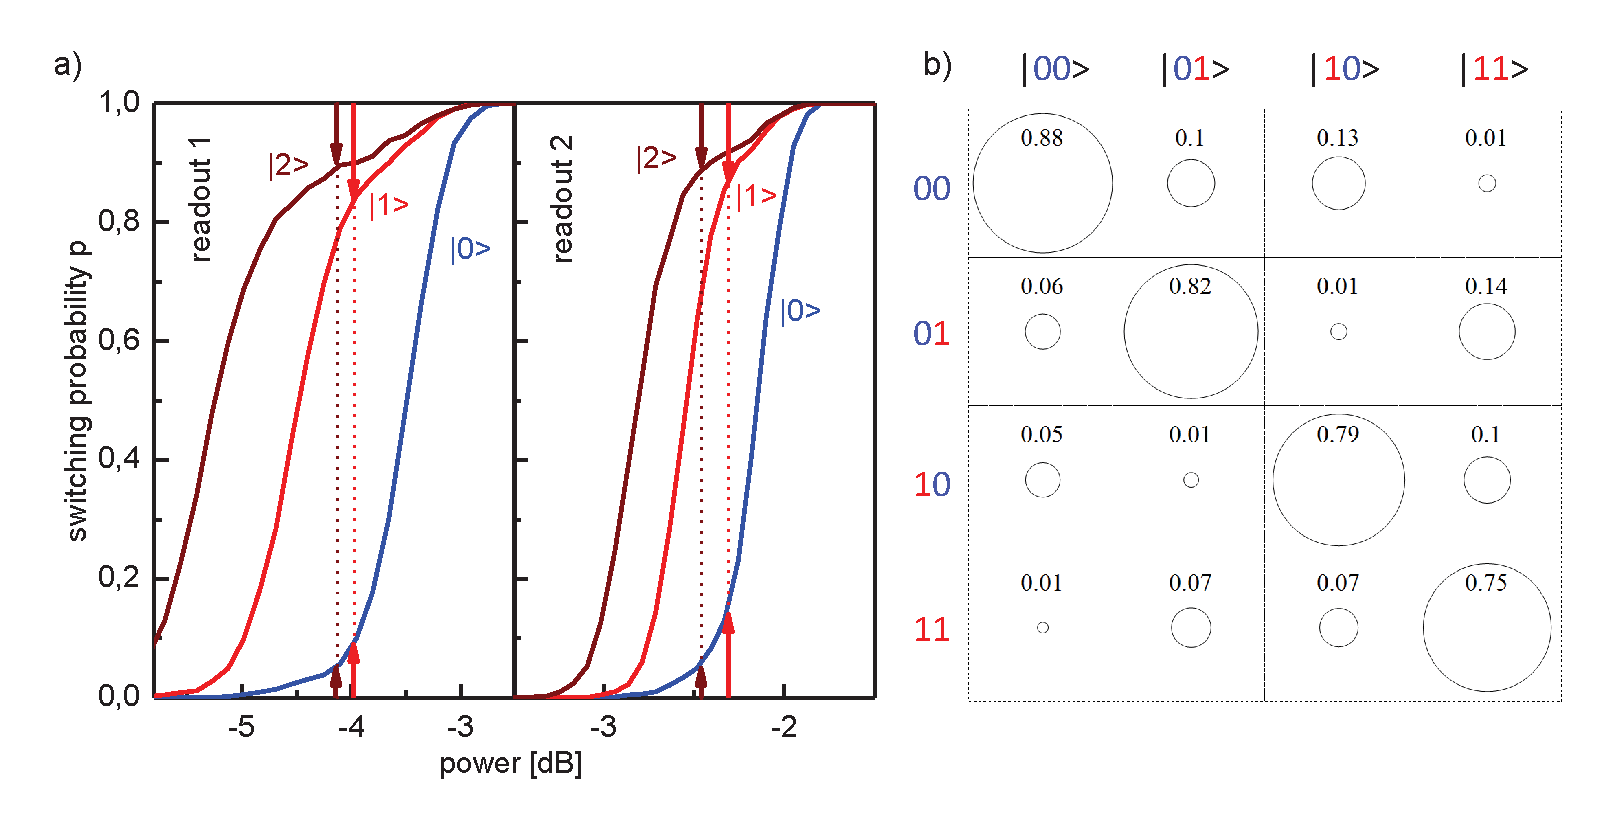
\includegraphics[width=1.\textwidth]{./material/papers/grover/figures/simultaneous_readout_characteristics}
	\caption[Switching probabilities of the two qubit readouts as a function of the readout excitation power]{a) Switching probabilities of the two qubit readouts as a function of the readout excitation power. The measurement is performed after preparing the qubits in the states $\color{blue}{\ket{0}}$, $\color{red}{\ket{1}}$ and $\color{brown}{\ket{2}}$. The readout fidelity is given as the difference in probability between the curves corresponding to the states $\color{blue}{\ket{0}}$ and $\color{red}{\ket{1}}$ or $\color{brown}{\ket{2}}$, respectively. The highest readout fidelites of 88 and 89 \% are achieved when the qubit is in state $\color{brown}{\ket{2}}$. b) Readout matrix of the two-qubit system. The matrix contains the probabilities of obtaining a given measurement result after having prepared the system in a given state. \figcomment{Replace this figure since it is not very intuitive. It would be better to show something which allows the reader to directly quantify the visibility and readout crosstalk present in the system.}}
	\label{fig:qubit_readout_characteristics}
\end{figure}

To read out the state of each qubit, a so-called Josephson bifurcation amplifier \citep{siddiqi_dispersive_2006,mallet_single-shot_2009} is used. This readout works by capacitively coupling the qubit to a coplanar waveguide resonator which is rendered nonlinear by adding a Josephson junction at its center. This nonlinear resonator can exhibit bistable behaviour for certain drive parameters, which we use to map the state of the qubit to one of the bistable states of the resonator, thus obtaining a single-shot readout of the qubit state. In contrast to other CQED architectures, in our approach each of the qubits possesses its own JBA readout, allowing a simultaneous measurement of the state of the whole qubit register, thus following closely the canonical blueprint of a quantum computer as formulated by DiVincenzo.\todo{discuss more details of the readout here...} Up to 93 \% readout fidelity has been demonstrated using the JBA readout \citep{mallet_single-shot_2009}, but due to design contraints the fidelity attained in the experiments discussed here was bound to 83-85 \% , as shown in fig. \ref{fig:qubit_readout_characteristics}. By measuring the simultaneous readout switching probabilities after initializing the qubit register in a given state we can extract and correct all readout errors.

\section{Generating and Characterizing Entanglement}

\begin{figure}
	\centering
		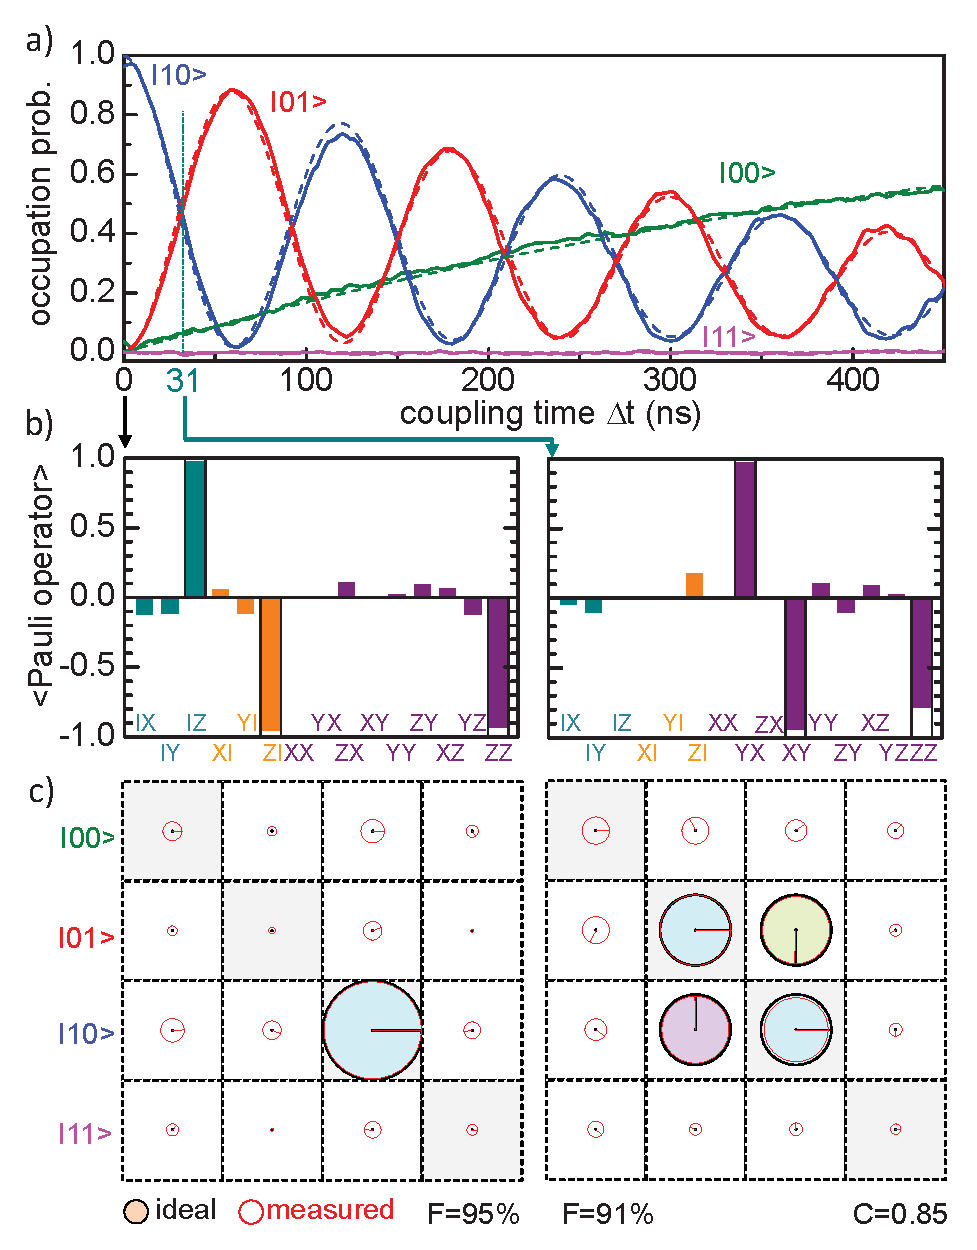
\includegraphics[width=0.7\textwidth]{./material/papers/iswap/submission1/Dewes_Figure2}
	\caption[Generating entangled two-qubit states by swapping interaction]{Energy oscillations between the two qubits induced by a resonant swapping interaction between them. a) The qubit state after switching on the swapping interaction for a given time $\Delta t$. The frequency of the oscillations corresponds to $2g = 8.7 \; \mathrm{MHz}$. b) The Pauli set of the two-qubit state measured at $0\; \mathrm{ns}$ and $31\; \mathrm{ns}$. c) The reconstructed density matrices corresponding to the two measured Pauli sets. In c), the area of each circle corresponds to the absolute value of each matrix element and the color and direction of the arrow give the phase of each element. The black circles correspond to the density matrices of the ideal states $\ket{10}$ and $1/\sqrt{2}/(\ket{10}+i\ket{01})$, respectively.\figcomment{verify sign!}}
	\label{fig:swap_interaction_state_tomography}
\end{figure}

The fixed coupling between the two qubits provides a $\sigma_{xx}$-type coupling which is only effective when the qubit frequencies are nearly resonant. Therefore, it can be switched on and off by changing the qubit frequencies, which we use to implement two-qubit gates with this system. In our processor, the effective coupling constant $g$ of the two qubits is given as $2g = 8.2 \; \mathrm{MHz}$\todo{Check if this is really $2g$!}. When using a fast fluxline pulse to abruptly tune the qubits in resonance we can switch on the qubit-qubit coupling non-adiabatically and generate an evolution operator of the form

\begin{equation}
	U(t)  =  \left( \begin{array}{cccc} 1 & 0 & 0 & 0 \\ 0 & \cos{2 \pi t g} & i\sin{2 \pi t g} & 0 \\ 0 & i\sin{2 \pi t g} & \cos{2 \pi t g} & 0 \\ 0 & 0 & 0 & 1 \end{array} \right) \label{eq:swap_evolution_operator}
\end{equation}

%explain that we stop the evolution at the right time to generate entangled states and implement a Two-qubit gate.

Switching off this interaction after a time $t_{\pi/2} = 1/8 g$ allows the creation of entangled qubit states and the implementation of a universal quantum gate, as will be explained later. Before doing this, we characterize the evoluation of the qubits during the swapping interaction by preparing them in the state $\ket{10}$, switching on the interaction for a given amount of time and measuring the qubit state directly afterwards. The resulting curve shown in fig. \ref{fig:swap_interaction_state_tomography} shows energy oscillations between the two qubits. Stopping the interaction after quarter of a period we obtain an entangled two-qubit Bell-type state that we can characterize by performing quantum state tomography. The experimental reconstruction of the density matrix of such a state corresponding approximating to the Bell-state $\ket{\psi} = 1/\sqrt{2}(\ket{01}+i\ket{10})$ is shown in fig. \ref{fig:swap_interaction_state_tomography}b. The measured fidelity of this state of 91 \% and the concurrence of 85 \% confirms that entanglement is present in the system. This entanglement can also be characterized by measuring the so-called {\it Clauser-Horne-Shimony-Holt} operator \citep{clauser_proposed_1969} on the produced state. This operator is given as

\begin{equation}
\mathrm{CHSH} = \mathrm{QS}+\mathrm{RS}+\mathrm{RT}-\mathrm{QT}
\end{equation}
with the operators $\mathrm{Q,R,S,T}$ being given as

\begin{eqnarray}
	\begin{array}{cccccccc}
		\mathrm{Q} & = & \sigma_z^1 &&& \mathrm{S} & = & \sigma_z^2\cdot \cos{\phi}+\sigma_x^2 \cdot \sin{\phi} \\
		\mathrm{R} & = & \sigma_x^1 &&& \mathrm{T} & = & -\sigma_z^2\cdot \sin{\phi}+\sigma_x^2 \cdot \cos{\phi}
	\end{array}
\end{eqnarray} 
Here, the angle $\phi$ is a parameter that should be chosen in accordance to the phase of the Bell state on which the operator is applied.

\begin{figure}[ht!]
	\centering
		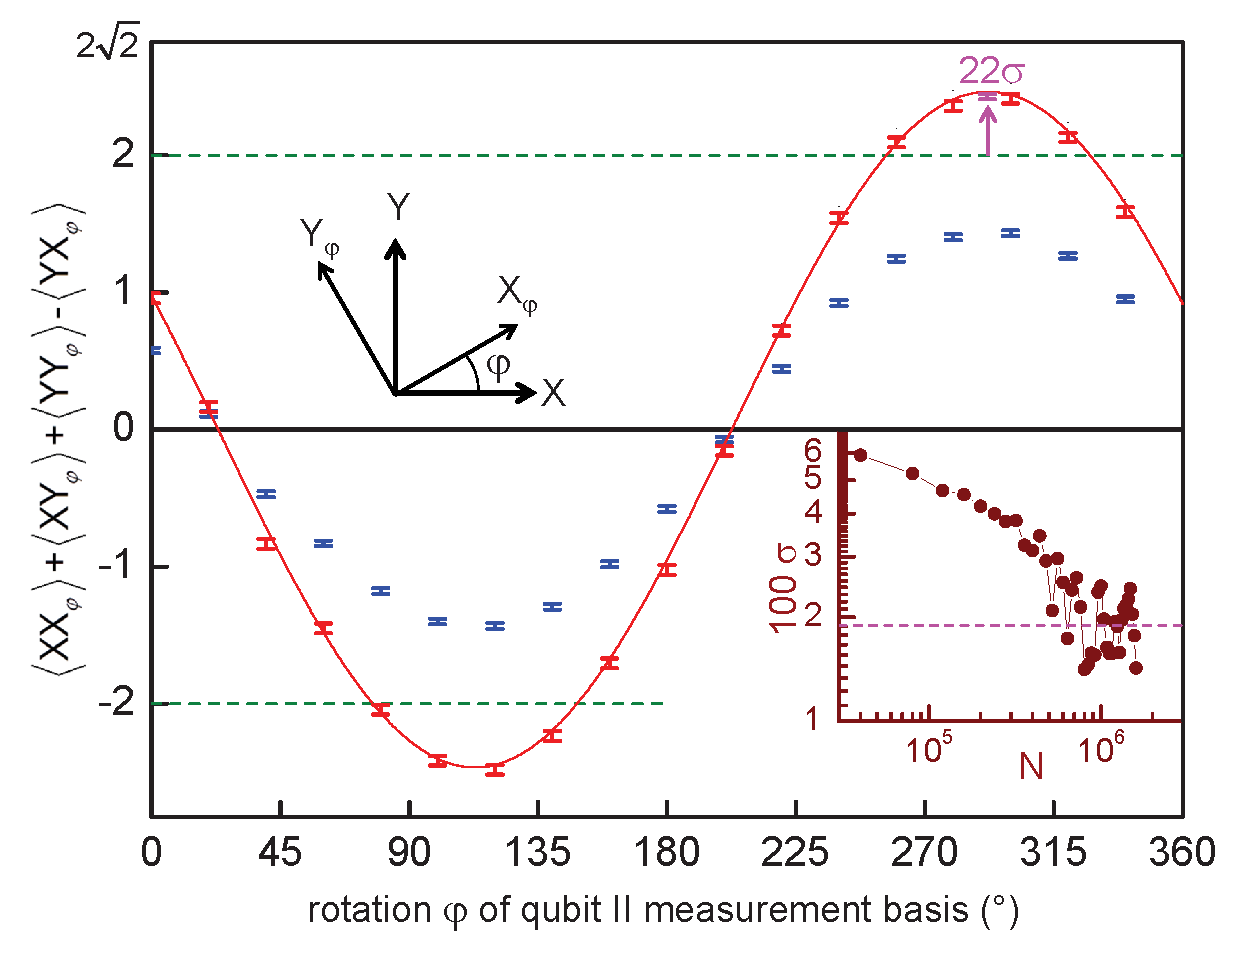
\includegraphics[width=0.7\textwidth]{./material/papers/iswap/submission1/Dewes_Figure3}
	\caption[Measurement of the CHSH operator of an entanged two-qubit state]{Measurement of the CHSH equation for an entangled two-qubit state. The renormalized CHSH expectation value (red points) exceeds the classical boundary of $2$ by a large amount. The raw measurement data (blue points) lies below this critical threshold. The inset shows the standard deviation $\sigma$ at the highest point of the curve as a function of the measurement sample size. For the highest sample count, the classical boundary is exceeded by $22$ standard deviations.\figcomment{p. 140 in cavities 6 labbook}}
	\label{fig:chsh_measurement}
\end{figure}

The expectation value $\bracket{CHSH}$ provides a test of the quantum-mechanical character of the generated state. For classical states, the maximum value is $\le 2$ but for entangled states it can reach a maximum value of $\sqrt{2}\cdot 2$. The result of a CHSH-type measurement performed on a state created by the method described above is shown in fig. \ref{fig:chsh_measurement}, showing the value of $\bracket{CHSH}$ as a function of $\phi$. We observe a violation of the classical boundary $2$ of the operator by $22$ standard deviations when correcting readout errors present in our system. However, the raw, uncorrected data fails to exceed the non-classical bound, making it impossible to close the detection loophole with our system. Nevertheless the observed violation of the equation by the renormalized state is a strong indication of entanglement in the system.

\section{Realizing a Universal Two-Qubit Quantum Gate}

\begin{SCfigure}[][ht!]
		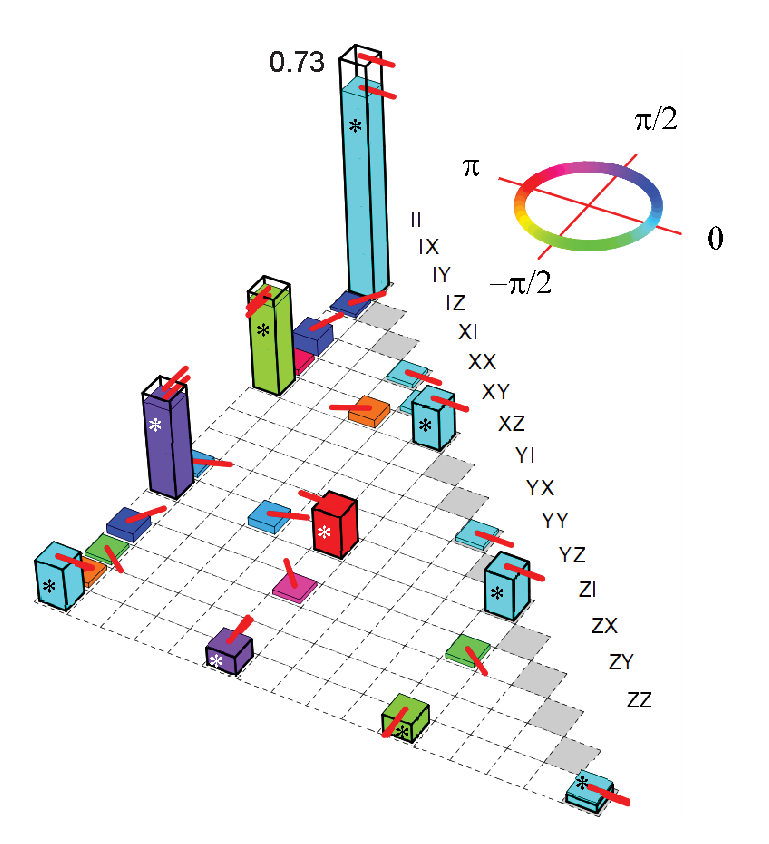
\includegraphics[width=0.65\textwidth]{./material/papers/iswap/figures/chi_matrix}
	\caption[Measured $\chi$-matrix of the $\sqrt{i\textrm{SWAP}}$ gate]{The measured $\chi$-matrix of the implemented $\sqrt{i\mathrm{SWAP}}$ gate. The row labels correspond to the indices of the $E_i$ operators, the height of each bar to the absolute value of the corresponding matrix element and the color and direction of the red arrow to the complex phase of each element. The ideal $\chi$-matrix of the $i\sqrt{\mathrm{SWAP}}$ gate is given by the outlined bars. The upper half of the positive-hermitian matrix is not shown.}
	\label{fig:gate_chi_matrix_and_errors}
\end{SCfigure}

The swapping evolution according to eq. (\ref{eq:swap_evolution_operator}) allows the implementation of a two-qubit gate. When switching on this interaction for $t_{\pi/2} = 1/8g$ we can realize the so-called $\sqrt{i\mathrm{SWAP}}$ gate, which has the representation

\begin{equation}
	\sqrt{i\mathrm{SWAP}}  =  \left( \begin{array}{cccc} 1 & 0 & 0 & 0 \\ 0 & 1/\sqrt{2} & i/\sqrt{2} & 0 \\ 0 & i/\sqrt{2} & 1/\sqrt{2} & 0 \\ 0 & 0 & 0 & 1 \end{array} \right) \label{eq:sqrt_iswap_gate}
\end{equation}
and is a universal two-qubit quantum gate. The operation and errors of our implementation of this gate can be characterized by performing quantum process tomography, yielding a gate fidelity of 90 \% . The 10 \% error in gate fidelity is caused mainly by qubit relaxation and dephasing during the gate operation and only marginally by deterministic preparation errors, as will be discussed in the main text of the thesis. Fig. \ref{fig:gate_chi_matrix_and_errors} show the measured $\chi$ matrix of the implemented gate. The achieved fidelity of the gate operation is sufficient to allow the implementation of a simple quantum algorithm with our processor, as will be discussed in the following section.
 
\section{Running a Quantum-Search Algorithm}

\begin{figure}[ht!]
	\centering
		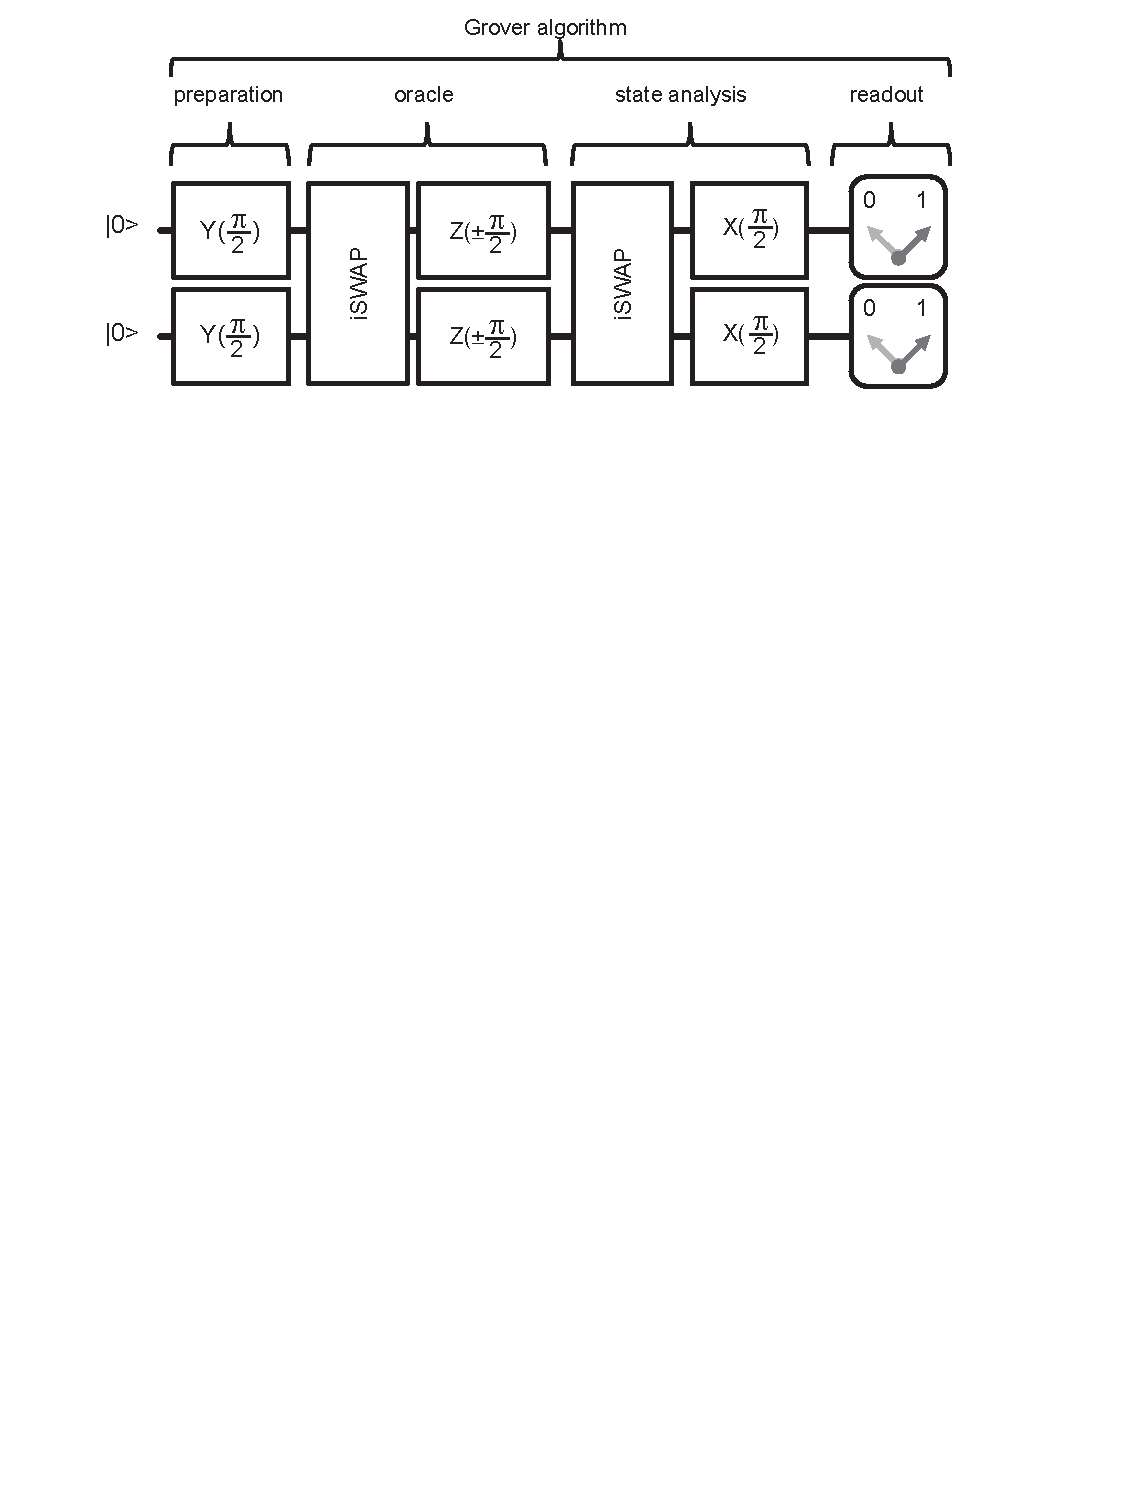
\includegraphics[width=0.8\textwidth]{./material/papers/grover/figures/grover_algorithm_schematic}
	\caption[Schematic of the implementation of Grovers search algorithm]{Schematic of the implementation of Grovers search algorithm on a two-qubit quantum processor. The algorithm consists in preparing a probe state, applying the quantum oracle to this state and analyzing the resulting output state to extract the information on the oracle operator.} 
	\label{fig:grover_algorithm_schematic}
\end{figure}

In this work we use the quantum gate implemented above to run a compiled version of Grover's search algorithm \citep{Grover_Quantum_1997}. The implemented version of the algorithm works in the basis of two qubits $x_i \in \{\ket{00},\ket{01},\ket{10},\ket{11}\}$ and  can distinguish between four different {\it oracle functions} $f(x)$ that each tag on one of the basis states $x_j$. Since the Grover algorithm for 2 qubits requires only one evaluation of the function $f(x)$ to determine which state has been marked it is faster than any conceivable classical algorithm, thus demonstrating the concept of quantum speed-up. The schematic of our version of Grover's algorithm is shown in fig. \ref{fig:grover_algorithm_schematic} and involves two $i\mathrm{SWAP}$ gates and three single-qubit operations along with a single-shot qubit readout at the end of the algorithm. We implemented all steps of this algorithm with our two-qubit processor and performed quantum state tomography after each step to reconstruct the quantum state at different points in the algorithm. Fig. \ref{fig:grover_density_matrices_state_1} shows the experimentially measured density matrices when running the algorithm with an oracle that marks the state $\ket{00}$. State tomographies are shown after applying the generalized Hadamard transform, after applying the quantum oracle and after the final step of the algorithm. This reconstruction of the quantum state using quantum state tomography does not however allow to demonstrate quantum speed-up, which requires individual single-shot readout of the qubit register, which will be discussed in the following section.

\begin{figure}[ht!]
	\centering
		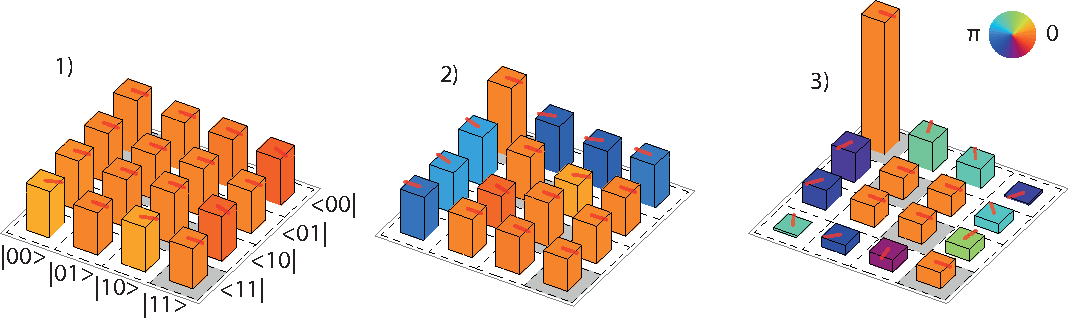
\includegraphics[width=1.\textwidth]{./material/figures/2-qubit-processor/grover/grover-density-matrices-state-1}
	\caption[Measured density matrices when running Grover's algorithm]{Measured density matrices when running Grover's search algorithm with a search oracle marking the state $\ket{00}$. 1) shows the state after the generalized Hadamard transform, 2) after applying the quantum oracle and 3) after the final step of Grover's algorithm.} 
	\label{fig:grover_density_matrices_state_1}
\end{figure}


\section{Demonstrating Quantum Speed-Up}

The main interest of running a quantum algorithm is to obtain an advantage in the run-time in comparision with a classical algorithm, the so-called {\it quantum speed-up}. To characterize this quantum speed-up as obtained with our processor, we run Grovers algorithm for all four possible oracle functions and directly readout out the qubit state after the last step of the algorithm, without correcting any readout errors. When averaging the results of such individual runs of the algorithm we can then obtain its single-run fidelity, which --for our processor-- ranges between 52 and 67 \%, depending on the state which is  marked by the quantum oracle, as shown in fig. \ref{fig:grover_single_shot_probabilities}. These results clearly demonstrate quantum speed-up in this system, although the achieved success probability is considerably lower than the theoretically possible value of 100 \% . The reduced fidelity is mainly due to relaxation and decoherence of the qubit state during the running of the algorithm and to a very small degree due to errors in the pulse sequence and drifts in the measurement equipment.

\begin{figure}[ht!]
		\centering
		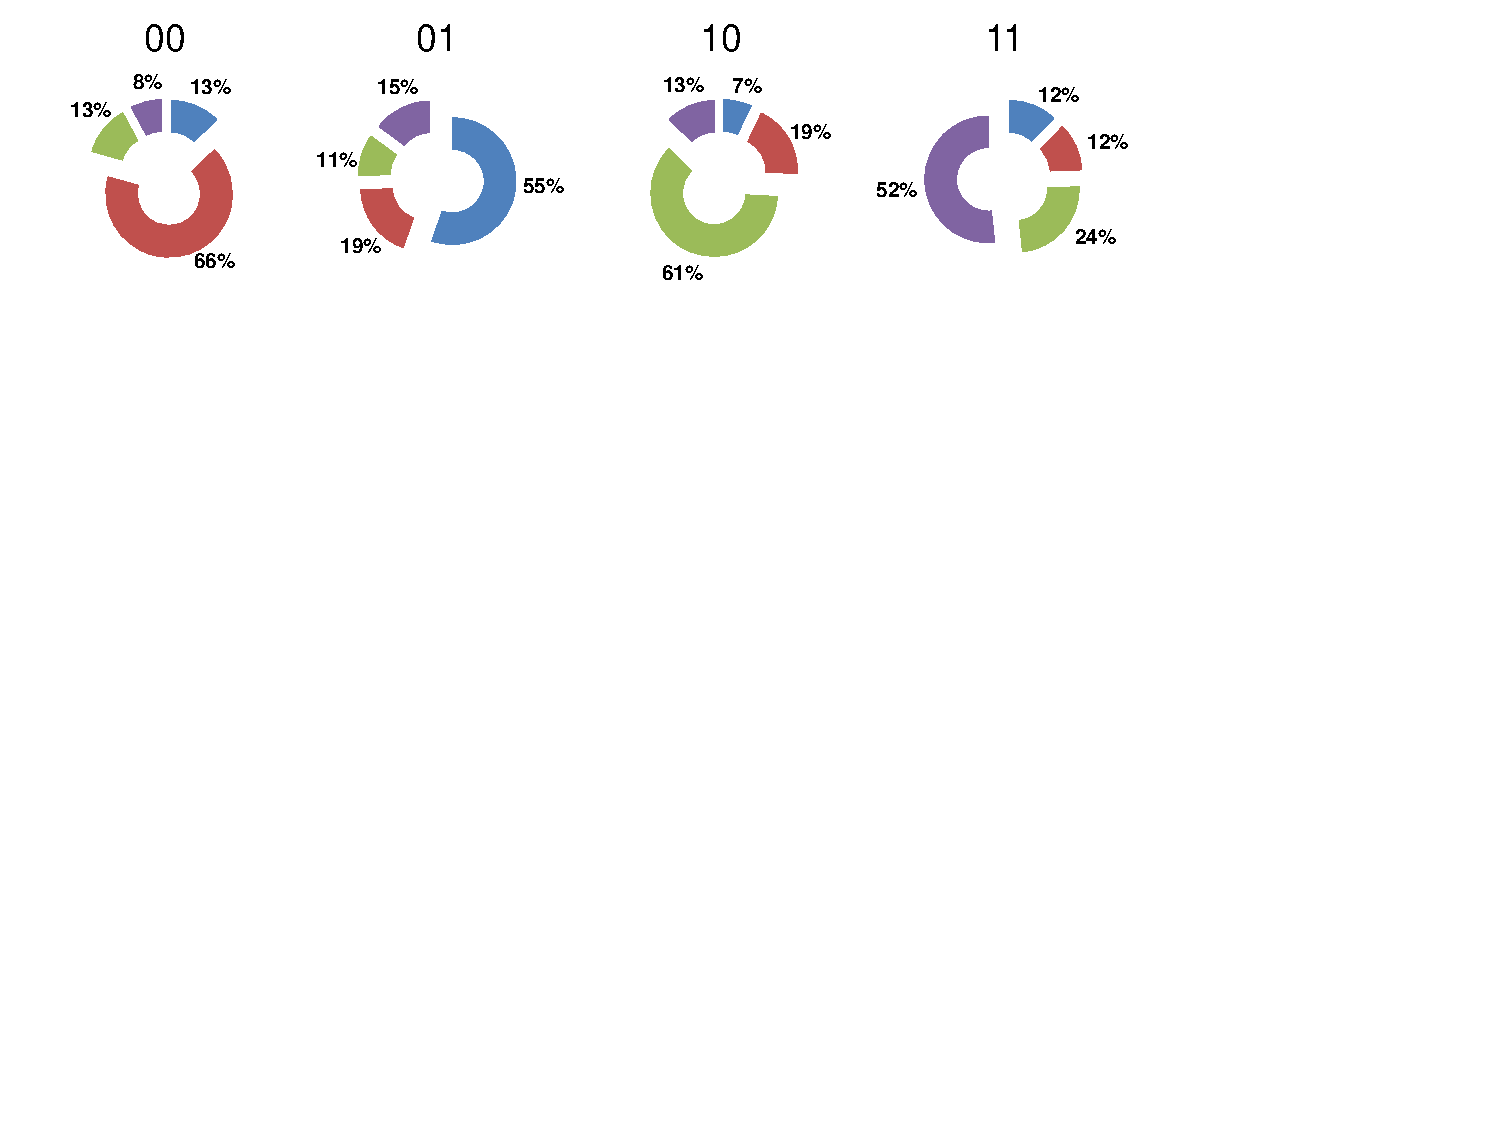
\includegraphics[width=1.0\textwidth]{./material/papers/grover/figures/grover_algorithm_single_shot_probabilities}
	\caption[Single-run results of the Grover search algorithm]{Single-run results when running the Grover search algorithm on our two-qubit quantum processor. Shown are the probabilities of obtaining the results $00,01,10,11$ as a function of the oracle function provided to the algorithm, indicated by the number on top of each graph. In all four cases, the success probability of the algorithm is $> 50 \%$, thus outperforming any classical algorithm in the number of calls to the oracle function.}
	\label{fig:grover_single_shot_probabilities}
\end{figure}

\section{Designing a Scalable Quantum Computing Architecture}

After having demonstrated the different building blocks of a superconducting, Transmon-based quantum processor it remains to be shown that larger-scale quantum-computing beyond two qubits is possible with this system. This work therefore pursued the realization of a more scalable qubit architecture using systems of up to six qubits coupled through a so-called ``quantum bus'' \citep{majer_coupling_2007}. The details of this novel architecture are discussed in the following sections.

The approach for scalable quantum computing with superconducting qubits pursued in this work consists of a system of many individual Transmon qubits equipped with individual JBA-based readouts, a multiplexed drive and readout circuit and a fixed qubit-qubit coupling mediated through a high-Q CPW resonator. As before, each qubit possesses a fluxline for fast frequency control. The readout and drive signals are send to all the qubits in parallel through a multiplexed transmission line. In this approach, the qubit and readout parameters, couplings and frequencies have to be carefully to avoid unwanted coupling between individual qubits and readouts and to allow the implementation of robust quantum gates between individual qubits. In this work we realized a 4-qubit chip and characterized it experimentally. The results of these experiments will be discussed in the main text of this thesis.

\begin{figure}[ht!]
  \centering
	\includegraphics[width=1.\textwidth]{"./material/figures/scalable-architecture/scalable architecture - schematic"}
	\caption[...]{...}
\end{figure}
